\section{Graphic interface}

\begin{figure}%
    \centering
    \subfloat[\centering Menu file]
    {{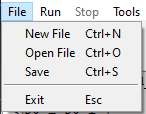
\includegraphics{images/menu/menu_file.png} }}%
    \qquad
    \subfloat[\centering Menu help]
    {{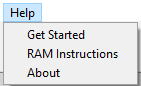
\includegraphics{images/menu/menu_help.png} }}%
    \qquad
    \subfloat[\centering Menu run]
    {{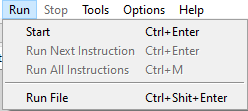
\includegraphics{images/menu/menu_run.png} }}%
    \qquad
    \subfloat[\centering Menu tools]
    {{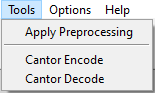
\includegraphics{images/menu/menu_tools.png} }}%
    \qquad
    \subfloat[\centering Menu option]
    {{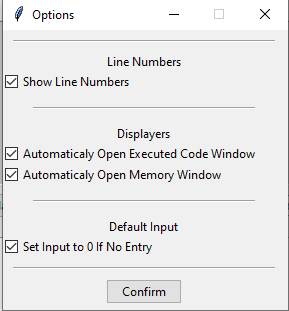
\includegraphics[width=5cm]{images/menu/menu_option.png} }}%
    \caption{Menu previews}%
    \label{fig:menu_images}%
\end{figure}

\subsection{Menu bar}
On the menu bar we can find :
\begin{itemize}
    \item \textbf{File}:
    \begin{itemize}
        \item \textit{New File} : Open a new blank file into a new tab (with an ephemeral default name, until you save it).
        \item \textit{Open File} : Choose and open an existing file with your OS file browser and load it.
        \item \textit{Save} : Save the current file on the disk. If it is a new created file, the name and save location will be asked.
        \item \textit{Exit} : Quit the application. Be careful to previously save
        your unsaved files before performing this action.
    \end{itemize}
    \item \textbf{Run}:
    \begin{itemize}
        \item \textit{Start} : Begin the sequential execution of the current file. This means that you start executing the first instruction, then you manually execute each of the following instructions. The program stops as soon as the last instruction has been executed.\\
        \textit{Remark: this command will be disabled if the sequential execution has already been started.}
        \item \textit{Run Next Instruction} : Execute the next instruction of the program.\\
        \textit{Remark: this command is disabled if the sequential execution hasn't already been started.}
        \item \textit{Run All Instructions} : Execute all the next instructions of the program. The delay between two execution is 0.1 sec.\\
        \textit{Remark: this command is disabled if the sequential execution hasn't already been started.}
        \item \textit{Run File} : Execute the whole file in one go.
    \end{itemize}
    \item \textbf{Stop}: Interrupt the current sequential execution. Memory will be reset.\\
    \textit{Remark: this command is disabled if the sequential execution hasn't already been started.}
    \item \textbf{Tools}:
    \begin{itemize}
        \item \textit{Apply Preprocessing} : Modify the current file by executing only the preprocessing instructions (\#define and \#include). It is useful
        when we got an error to see the involved line or to see the final program which will be parsed.
        \item \textit{Cantor Encode} : Open a utility window in which you can convert two integers to one with the Cantor's function.
        \item \textit{Cantor Decode} : Like the previous command, but the reverse function.
    \end{itemize}
    \item \textbf{Options}: Open the settings window in which we can check/uncheck:
    \begin{itemize}
        \item Show the lines numbers of the text editor
        \item Automatically open the executed code's window
        \item Automatically open the memory's window
        \item Put the default value 0 if there is no R0 entry
    \end{itemize}
    You have to confirm to save and apply your choices. These will be saved on an JSON file.
    \item \textbf{Help}:
    \begin{itemize}
        \item \textit{Get Started}: Open an window in which the main command are explain. This is a user manual.
        \item \textit{RAM instructions}: Explanation of the four different RAM instructions.
        \item \textit{About}: Developers of the application.
    \end{itemize}
\end{itemize}

\subsection{Icons bar}

\begin{figure}[h]%
    \centering
    
\includegraphics{images/menu/menu_icons.png}%
    \caption{Icon bar}%
    \label{fig:icon_bar}%
\end{figure}

The icon bar (Figure \ref{fig:icon_bar}) is composed of four icons. The first one is a shortcut to save the current file. The second run the whole file, the third start the sequential execution and the last is the Stop shortcut.

\subsection{Text editor}

This widget is where you can write and edit your code. This is also here the file you open will be loaded.
Line numbers are displayed to the left of the text entry field.

\subsection{Entry}

You can set the value of the R0 register when you run the program. If no value is entered, an error message will be displayed, except if you set the adequate option.
\subsection{Displayers}
Two windows are available to see and debug your RAM program. The first (\textit{Display Executed Code}) displays all the instructions after the preprocessing and parsing phases. If you execute a code sequentially, the last executed instruction will be highlighted. Since then, you can easily see and debug the progress of the program.

The second one (\textit{Display Memory}) will display the state of the memory (registers). Equally, the memory will be actualize to each iterations.
Each window is assigned to a file.
\subsection{Output console}
It is in this terminal that you will see the file execution's result. Error messages will also be displayed there.
If the program contains a grammatical error or an unrecognized instruction, the file will not be interpreted and the number of the line on which the said error appears will be displayed. Attention, this is the line corresponding to the preprocessed file.
You can adjust the space taken by it easily by hovering the mouse just below the widget where the code is inserted, as you would with a window.
\subsection{Shortcuts}
Several shortcut allow you to perform action quickly.

\underline{Inside the text editor:}
\begin{itemize}
    \item \textbf{\textit{Ctrl+Shit+Enter}} : Run whole file.
    \item \textbf{\textit{Ctrl+Enter}} : Start sequential execution.
    \item \textbf{\textit{Ctrl+M}} : Run all instructions sequentially.
    \item \textbf{\textit{Right-Click}} : Show contextual menu.
\end{itemize}
Depending on whether you are in RAM program or Int code mode, the right-click contextual menu changes.\\
In \textbf{RAM Program mode}, you can mark a line as the end of file when you run it. You can remove the marker.
You also have the possibility of executing the file directly from this contextual menu.\\
In \textbf{Int Code mode}, you will be offered to convert the file that contains the int to a RAM program in a new tab, or you can directly execute the int.


\underline{On the main window:}
\begin{itemize}
    \item \textbf{\textit{Ctrl+S}} : Save the current file.
    \item \textbf{\textit{Ctrl+O}} : Open file.
    \item \textbf{\textit{Ctrl+N}} : Create new file.
    \item \textbf{\textit{Esc}} : Exit
\end{itemize}


\begin{figure}[t]%
    \centering
    \subfloat[\centering Main panel]
    {{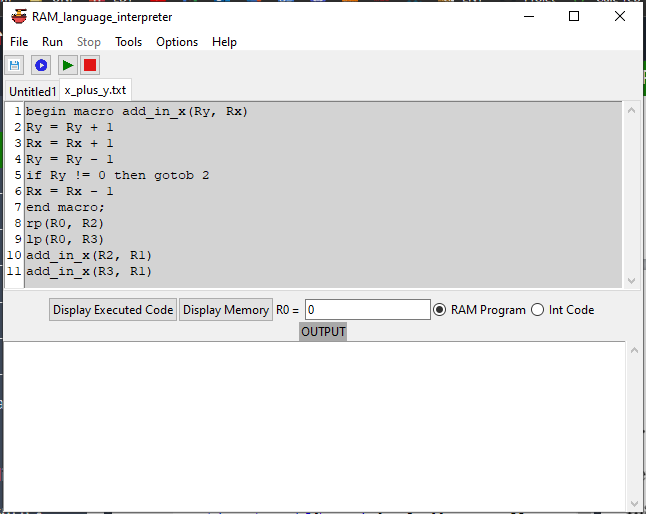
\includegraphics[width=8cm]{images/gui.png} }}%
    \qquad
    \subfloat[\centering Memory panel]
    {{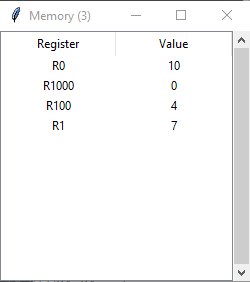
\includegraphics[width=4cm]{images/memory.png} }}%
    \caption{Example of our graphic interface}%
    \label{fig:gui}%
\end{figure}
